
%% bare_conf.tex
%% V1.4b
%% 2015/08/26
%% by Michael Shell
%% See:
%% http://www.michaelshell.org/
%% for current contact information.
%%
%% This is a skeleton file demonstrating the use of IEEEtran.cls
%% (requires IEEEtran.cls version 1.8b or later) with an IEEE
%% conference paper.
%%
%% Support sites:
%% http://www.michaelshell.org/tex/ieeetran/
%% http://www.ctan.org/pkg/ieeetran
%% and
%% http://www.ieee.org/

%%*************************************************************************
%% Legal Notice:
%% This code is offered as-is without any warranty either expressed or
%% implied; without even the implied warranty of MERCHANTABILITY or
%% FITNESS FOR A PARTICULAR PURPOSE! 
%% User assumes all risk.
%% In no event shall the IEEE or any contributor to this code be liable for
%% any damages or losses, including, but not limited to, incidental,
%% consequential, or any other damages, resulting from the use or misuse
%% of any information contained here.
%%
%% All comments are the opinions of their respective authors and are not
%% necessarily endorsed by the IEEE.
%%
%% This work is distributed under the LaTeX Project Public License (LPPL)
%% ( http://www.latex-project.org/ ) version 1.3, and may be freely used,
%% distributed and modified. A copy of the LPPL, version 1.3, is included
%% in the base LaTeX documentation of all distributions of LaTeX released
%% 2003/12/01 or later.
%% Retain all contribution notices and credits.
%% ** Modified files should be clearly indicated as such, including  **
%% ** renaming them and changing author support contact information. **
%%*************************************************************************


% *** Authors should verify (and, if needed, correct) their LaTeX system  ***
% *** with the testflow diagnostic prior to trusting their LaTeX platform ***
% *** with production work. The IEEE's font choices and paper sizes can   ***
% *** trigger bugs that do not appear when using other class files.       ***                          ***
% The testflow support page is at:
% http://www.michaelshell.org/tex/testflow/



\documentclass[conference]{IEEEtran}
% Some Computer Society conferences also require the compsoc mode option,
% but others use the standard conference format.
%
% If IEEEtran.cls has not been installed into the LaTeX system files,
% manually specify the path to it like:
% \documentclass[conference]{../sty/IEEEtran}





% Some very useful LaTeX packages include:
% (uncomment the ones you want to load)


% *** MISC UTILITY PACKAGES ***
%
%\usepackage{ifpdf}
% Heiko Oberdiek's ifpdf.sty is very useful if you need conditional
% compilation based on whether the output is pdf or dvi.
% usage:
% \ifpdf
%   % pdf code
% \else
%   % dvi code
% \fi
% The latest version of ifpdf.sty can be obtained from:
% http://www.ctan.org/pkg/ifpdf
% Also, note that IEEEtran.cls V1.7 and later provides a builtin
% \ifCLASSINFOpdf conditional that works the same way.
% When switching from latex to pdflatex and vice-versa, the compiler may
% have to be run twice to clear warning/error messages.






% *** CITATION PACKAGES ***
%
%\usepackage{cite}
% cite.sty was written by Donald Arseneau
% V1.6 and later of IEEEtran pre-defines the format of the cite.sty package
% \cite{} output to follow that of the IEEE. Loading the cite package will
% result in citation numbers being automatically sorted and properly
% "compressed/ranged". e.g., [1], [9], [2], [7], [5], [6] without using
% cite.sty will become [1], [2], [5]--[7], [9] using cite.sty. cite.sty's
% \cite will automatically add leading space, if needed. Use cite.sty's
% noadjust option (cite.sty V3.8 and later) if you want to turn this off
% such as if a citation ever needs to be enclosed in parenthesis.
% cite.sty is already installed on most LaTeX systems. Be sure and use
% version 5.0 (2009-03-20) and later if using hyperref.sty.
% The latest version can be obtained at:
% http://www.ctan.org/pkg/cite
% The documentation is contained in the cite.sty file itself.

\usepackage{graphicx}


% *** GRAPHICS RELATED PACKAGES ***
%
%\ifCLASSINFOpdf
  %\usepackage[pdftex]{graphicx}
  % declare the path(s) where your graphic files are
  % \graphicspath{{../pdf/}{../jpeg/}}
  % and their extensions so you won't have to specify these with
  % every instance of \includegraphics
  % \DeclareGraphicsExtensions{.pdf,.jpeg,.png}
%\else
  % or other class option (dvipsone, dvipdf, if not using dvips). graphicx
  % will default to the driver specified in the system graphics.cfg if no
  % driver is specified.
  % \usepackage[dvips]{graphicx}
  % declare the path(s) where your graphic files are
  % \graphicspath{{../eps/}}
  % and their extensions so you won't have to specify these with
  % every instance of \includegraphics
  % \DeclareGraphicsExtensions{.eps}
%\fi
% graphicx was written by David Carlisle and Sebastian Rahtz. It is
% required if you want graphics, photos, etc. graphicx.sty is already
% installed on most LaTeX systems. The latest version and documentation
% can be obtained at: 
% http://www.ctan.org/pkg/graphicx
% Another good source of documentation is "Using Imported Graphics in
% LaTeX2e" by Keith Reckdahl which can be found at:
% http://www.ctan.org/pkg/epslatex
%
% latex, and pdflatex in dvi mode, support graphics in encapsulated
% postscript (.eps) format. pdflatex in pdf mode supports graphics
% in .pdf, .jpeg, .png and .mps (metapost) formats. Users should ensure
% that all non-photo figures use a vector format (.eps, .pdf, .mps) and
% not a bitmapped formats (.jpeg, .png). The IEEE frowns on bitmapped formats
% which can result in "jaggedy"/blurry rendering of lines and letters as
% well as large increases in file sizes.
%
% You can find documentation about the pdfTeX application at:
% http://www.tug.org/applications/pdftex





% *** MATH PACKAGES ***
%
\usepackage{amsmath}
% A popular package from the American Mathematical Society that provides
% many useful and powerful commands for dealing with mathematics.
%
% Note that the amsmath package sets \interdisplaylinepenalty to 10000
% thus preventing page breaks from occurring within multiline equations. Use:
%\interdisplaylinepenalty=2500
% after loading amsmath to restore such page breaks as IEEEtran.cls normally
% does. amsmath.sty is already installed on most LaTeX systems. The latest
% version and documentation can be obtained at:
% http://www.ctan.org/pkg/amsmath


\usepackage{mathrsfs}



% *** SPECIALIZED LIST PACKAGES ***
%
%\usepackage{algorithmic}
% algorithmic.sty was written by Peter Williams and Rogerio Brito.
% This package provides an algorithmic environment fo describing algorithms.
% You can use the algorithmic environment in-text or within a figure
% environment to provide for a floating algorithm. Do NOT use the algorithm
% floating environment provided by algorithm.sty (by the same authors) or
% algorithm2e.sty (by Christophe Fiorio) as the IEEE does not use dedicated
% algorithm float types and packages that provide these will not provide
% correct IEEE style captions. The latest version and documentation of
% algorithmic.sty can be obtained at:
% http://www.ctan.org/pkg/algorithms
% Also of interest may be the (relatively newer and more customizable)
% algorithmicx.sty package by Szasz Janos:
% http://www.ctan.org/pkg/algorithmicx




% *** ALIGNMENT PACKAGES ***
%
%\usepackage{array}
% Frank Mittelbach's and David Carlisle's array.sty patches and improves
% the standard LaTeX2e array and tabular environments to provide better
% appearance and additional user controls. As the default LaTeX2e table
% generation code is lacking to the point of almost being broken with
% respect to the quality of the end results, all users are strongly
% advised to use an enhanced (at the very least that provided by array.sty)
% set of table tools. array.sty is already installed on most systems. The
% latest version and documentation can be obtained at:
% http://www.ctan.org/pkg/array


% IEEEtran contains the IEEEeqnarray family of commands that can be used to
% generate multiline equations as well as matrices, tables, etc., of high
% quality.




% *** SUBFIGURE PACKAGES ***
%\ifCLASSOPTIONcompsoc
%  \usepackage[caption=false,font=normalsize,labelfont=sf,textfont=sf]{subfig}
%\else
%  \usepackage[caption=false,font=footnotesize]{subfig}
%\fi
% subfig.sty, written by Steven Douglas Cochran, is the modern replacement
% for subfigure.sty, the latter of which is no longer maintained and is
% incompatible with some LaTeX packages including fixltx2e. However,
% subfig.sty requires and automatically loads Axel Sommerfeldt's caption.sty
% which will override IEEEtran.cls' handling of captions and this will result
% in non-IEEE style figure/table captions. To prevent this problem, be sure
% and invoke subfig.sty's "caption=false" package option (available since
% subfig.sty version 1.3, 2005/06/28) as this is will preserve IEEEtran.cls
% handling of captions.
% Note that the Computer Society format requires a larger sans serif font
% than the serif footnote size font used in traditional IEEE formatting
% and thus the need to invoke different subfig.sty package options depending
% on whether compsoc mode has been enabled.
%
% The latest version and documentation of subfig.sty can be obtained at:
% http://www.ctan.org/pkg/subfig




% *** FLOAT PACKAGES ***
%
%\usepackage{fixltx2e}
% fixltx2e, the successor to the earlier fix2col.sty, was written by
% Frank Mittelbach and David Carlisle. This package corrects a few problems
% in the LaTeX2e kernel, the most notable of which is that in current
% LaTeX2e releases, the ordering of single and double column floats is not
% guaranteed to be preserved. Thus, an unpatched LaTeX2e can allow a
% single column figure to be placed prior to an earlier double column
% figure.
% Be aware that LaTeX2e kernels dated 2015 and later have fixltx2e.sty's
% corrections already built into the system in which case a warning will
% be issued if an attempt is made to load fixltx2e.sty as it is no longer
% needed.
% The latest version and documentation can be found at:
% http://www.ctan.org/pkg/fixltx2e


%\usepackage{stfloats}
% stfloats.sty was written by Sigitas Tolusis. This package gives LaTeX2e
% the ability to do double column floats at the bottom of the page as well
% as the top. (e.g., "\begin{figure*}[!b]" is not normally possible in
% LaTeX2e). It also provides a command:
%\fnbelowfloat
% to enable the placement of footnotes below bottom floats (the standard
% LaTeX2e kernel puts them above bottom floats). This is an invasive package
% which rewrites many portions of the LaTeX2e float routines. It may not work
% with other packages that modify the LaTeX2e float routines. The latest
% version and documentation can be obtained at:
% http://www.ctan.org/pkg/stfloats
% Do not use the stfloats baselinefloat ability as the IEEE does not allow
% \baselineskip to stretch. Authors submitting work to the IEEE should note
% that the IEEE rarely uses double column equations and that authors should try
% to avoid such use. Do not be tempted to use the cuted.sty or midfloat.sty
% packages (also by Sigitas Tolusis) as the IEEE does not format its papers in
% such ways.
% Do not attempt to use stfloats with fixltx2e as they are incompatible.
% Instead, use Morten Hogholm'a dblfloatfix which combines the features
% of both fixltx2e and stfloats:
%
% \usepackage{dblfloatfix}
% The latest version can be found at:
% http://www.ctan.org/pkg/dblfloatfix




% *** PDF, URL AND HYPERLINK PACKAGES ***
%
%\usepackage{url}
% url.sty was written by Donald Arseneau. It provides better support for
% handling and breaking URLs. url.sty is already installed on most LaTeX
% systems. The latest version and documentation can be obtained at:
% http://www.ctan.org/pkg/url
% Basically, \url{my_url_here}.




% *** Do not adjust lengths that control margins, column widths, etc. ***
% *** Do not use packages that alter fonts (such as pslatex).         ***
% There should be no need to do such things with IEEEtran.cls V1.6 and later.
% (Unless specifically asked to do so by the journal or conference you plan
% to submit to, of course. )

% *** Pseudocode PACKAGES ***
\usepackage{amsmath}
\DeclareMathOperator*{\argmin}{arg\,min}
\DeclareMathOperator*{\argmax}{arg\,max}
\usepackage{algorithm}
\usepackage{varwidth}
\usepackage[noend]{algpseudocode}
\makeatletter
\def\BState{\State\hskip-\ALG@thistlm}
\makeatother


\newcommand\NB[1]{$\spadesuit$\footnote{NB: #1}}
\newcommand\RP[1]{$\clubsuit$\footnote{RP: #1}}
% reference package for bibtex

%\usepackage{biblatex}
%\addbibresource{mybibliography.bib}

%\usepackage[
%backend=biber,
%style=numeric,
%sorting=ynt
%]{biblatex}

%\addbibresource{mybibliography.bib}


% correct bad hyphenation here
\hyphenation{op-tical net-works semi-conduc-tor}


\begin{document}
%
% paper title
% Titles are generally capitalized except for words such as a, an, and, as,
% at, but, by, for, in, nor, of, on, or, the, to and up, which are usually
% not capitalized unless they are the first or last word of the title.
% Linebreaks \\ can be used within to get better formatting as desired.
% Do not put math or special symbols in the title.
\title{Using Hidden Markov Models to Improve Autonomous Vehicle Decision Making - Problem Formulation}


% author names and affiliations
% use a multiple column layout for up to three different
% affiliations
\author{\IEEEauthorblockN{Rahul Peddi}
\IEEEauthorblockA{Systems and Information Engineering\\
University of Virginia\\
Charlottesville, Virginia\\
Email: rp3cy@virginia.edu}}

% conference papers do not typically use \thanks and this command
% is locked out in conference mode. If really needed, such as for
% the acknowledgment of grants, issue a \IEEEoverridecommandlockouts
% after \documentclass

% for over three affiliations, or if they all won't fit within the width
% of the page, use this alternative format:
% 
%\author{\IEEEauthorblockN{Michael Shell\IEEEauthorrefmark{1},
%Homer Simpson\IEEEauthorrefmark{2},
%James Kirk\IEEEauthorrefmark{3}, 
%Montgomery Scott\IEEEauthorrefmark{3} and
%Eldon Tyrell\IEEEauthorrefmark{4}}
%\IEEEauthorblockA{\IEEEauthorrefmark{1}School of Electrical and Computer Engineering\\
%Georgia Institute of Technology,
%Atlanta, Georgia 30332--0250\\ Email: see http://www.michaelshell.org/contact.html}
%\IEEEauthorblockA{\IEEEauthorrefmark{2}Twentieth Century Fox, Springfield, USA\\
%Email: homer@thesimpsons.com}
%\IEEEauthorblockA{\IEEEauthorrefmark{3}Starfleet Academy, San Francisco, California 96678-2391\\
%Telephone: (800) 555--1212, Fax: (888) 555--1212}
%\IEEEauthorblockA{\IEEEauthorrefmark{4}Tyrell Inc., 123 Replicant Street, Los Angeles, California 90210--4321}}




% use for special paper notices
%\IEEEspecialpapernotice{(Invited Paper)}




% make the title area
\maketitle

% As a general rule, do not put math, special symbols or citations
% in the abstract
\begin{abstract}
\end{abstract}

% no keywords




% For peer review papers, you can put extra information on the cover
% page as needed:
% \ifCLASSOPTIONpeerreview
% \begin{center} \bfseries EDICS Category: 3-BBND \end{center}
% \fi
%
% For peerreview papers, this IEEEtran command inserts a page break and
% creates the second title. It will be ignored for other modes.
\IEEEpeerreviewmaketitle



\section{Introduction}
% no \IEEEPARstart
    Over the last few years, semi-autonomous and autonomous vehicles have become increasingly popular, but they have not replaced traditional vehicles entirely just yet. This leads to a hybrid environment; one that features vehicles of all levels of autonomy. Many of these vehicles to be equipped with some form of adaptive cruise control (ACC) or advance driver assistance systems (ADAS), both of which help the driver make safe decisions while operating the vehicle. These types of systems are forms of human-robot interaction. ACC performs actions autonomously and works at the command of a human who determines a target velocity and a safe following distance. ADAS, on the contrary, acts as an information system for human drivers. These systems, however, are limited in their capabilities as they require constant monitoring from the driver and are unable to predict if the driver will enter a dangerous situation in the future. In addition, these systems can fail to guarantee safety in rapidly transitioning environments.
    
    One such example of an environment in which dangers arise rapidly are highways. Highways are often comprised of multiple lanes and many drivers performing different behaviors including lane changes, merges, passing, and reacting to other vehicles. In addition, highways involve traveling at very high velocities, which increase the likelihood that a dangerous situation will arise. \NB{I would keep this more general. We don't want to have a paper about highway safety. The highway should be an example}
    
    Because these dangerous situations can occur so rapidly \NB{need citation here}, there is a need to increase the ability to guarantee safety when developing new systems \NB{what do you mean with new systems?} for human drivers. This can be done by increasing the ability to predict and adapt to what will happen in the future. A simple depiction of a danger situation is shown in Fig. \ref{fig:hiway}. \NB{figure needs improvements}

\begin{figure}[ht]
    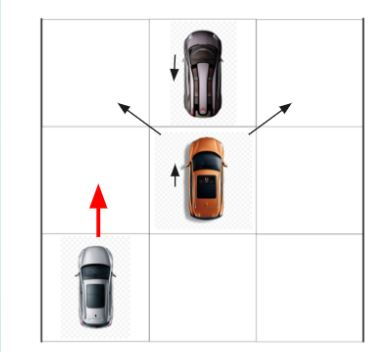
\includegraphics[width=0.5\textwidth]{highwaysit.JPG}
    \caption{Potentially dangerous highway situation. The vehicle in the center of the grid is the host vehicle, and the vehicle in front is driving much slower, while the vehicle to the right is approaching very rapidly. It would be safe in the instant to pass on the left, but that leaves the possibility that a dangerous situation will occur very soon.}
    \label{fig:hiway}
\end{figure}
    
    In terms of the adaptation, the human driver does control the vehicle, but it is important to have to ability to intervene and adjust the driver's actions as a dangerous situation arises. In this work, we aim to provide
    \begin{itemize}
    \item{a prediction method that can effectively and efficiently estimate the future positions of surrounding agents}
    \item{an adaptive framework that determines the adjustment and severity of such adjustment that should be made at any point in time}
    \end{itemize}
  
  \NB{we should briefly mention how we solve these problems here}  
    The rest of this paper is organized as follows: in Section II, we discuss related work, and in Section III, we formally define the problem. The method to predict future behaviors and positions of other vehicles are presented in Section IV. We demonstrate our results with simulations and experiments in Sections V and VI, respectively.Lastly, we discuss our conclusions and discuss future work in Section VII.

    
% You must have at least 2 lines in the paragraph with the drop letter
% (should never be an issue)

\section{Related Work}

%    This work is tuned a relatively specific situation; one where the host vehicle is driving in the middle lane of a three-lane highway. This was chosen in order to account for a large action space. In this case, there are three possible actions the host vehicle could take, and each of these actions is evaluated for safety. The action space is defined such that it only looks at the immediately adjacent lanes. For example, if the vehicle is in the left lane, the action space consists of forward, and move right. In this case, only those two actions are evaluated for safety at a future time step.
    
    
%    A Hidden Markov Model is a type of Markov Model, where the states are hidden. A Markov Model examines states and transitions to and from these states. An HMM operates on the assumption that we don't directly know what the state is, but we are able to make observations that can tell us valuable information about the current state. Hidden Markov Models have been used for many human-robot interaction applications \cite{li2016modeling}, including but not limited to speech recognition, motion recognition, and biological analyses \cite{yoon2009hidden}.
    
%    In addition to the host vehicle at the center of the road, there are two additional vehicles; one passing on the left lane, and a slowed vehicle ahead in the center lane, as shown in Figure \ref{fig:actionspace}.
    
%    The HMM was performed on the blue vehicle to the left (the purple vehicle is a representation of the estimate), from the perspective of the black vehicle, the host vehicle. The testing was done such that only one vehicle was able to make estimations, but in a truly hybrid environment, multiple vehicles will this technique will improve the ability for multiple vehicles to collaborate.
    
\section{Problem Formulation}
 
\textbf{Problem 1: \textit{Proactive Safe Assisted Planning and Control}:} 
    
    A human-operated vehicle $i$ is moving in an environment in the presence of stationary obstacles and other vehicles $j \in S_i(t)$, where $S_i(t)$ is a time varying set of vehicles in sensing/communication range with $i$. The goal is to find a policy to:
    \begin{enumerate}
        \item  predict online future states of the surrounding vehicles:
    \begin{equation}
    X_j={x_j(t), x_j(t+1),..., x_j(t+T)} \text{ with } j \in S_i(t)
    \end{equation}
    and assess their likelihood:
    \begin{equation}
    P_j={p_j(t), p_j(t+1),..., p_j(t+T)}
    \end{equation}
    \item assess the risk $0<= r_i <=1$ of a collision during $T$ and
    \item assist and intervene to correct the human-operated actions to guarantee safety, i.e., obtain an input $u_i$ such that if $r_i>\rho, \forall j \in S$ and for 
    \begin{equation}
    t<=T |x_i(t)-x_j(t)|>=d_{min} \text{ where } x_i(t)
    \end{equation}
    is the state of the human-operated vehicle at time $t$, $\rho$ is a user defined minimum risk threshold and $d_{min}$ is a minimum safe distance.

    \end{enumerate}

\section{Approach}


\subsection{System Model}
Include Dynamics? 

Block Diagram

\subsection{Training Models Using Hidden Markov Model}
In this section, we outline the Hidden Markov Model and training procedures used to obtain the models, with which we are able to make predictions about the future states of $j$.

A Hidden Markov Model (HMM) is an effective way to model sequential data where future states are generally unknown. HMMs consist of a set of $n$ states, $Q = q_1,q_2,...q_n$, a $n\times n$ \RP{Is this the best way to say this?} transition probability matrix, $A = a_{11},a_{12},...a_{n1},...a_{nn}$, where $n$ is the total number of states, a sequence of $m$ observations, $O = o_1,o_2,...o_m$, and a $n\times m$ matrix of observation likelihoods, $B = b_n(o_m)$. 

The general pictorial representation of an HMM is shown in Fig.\ref{fig:hmm}.
\begin{figure}[ht]
    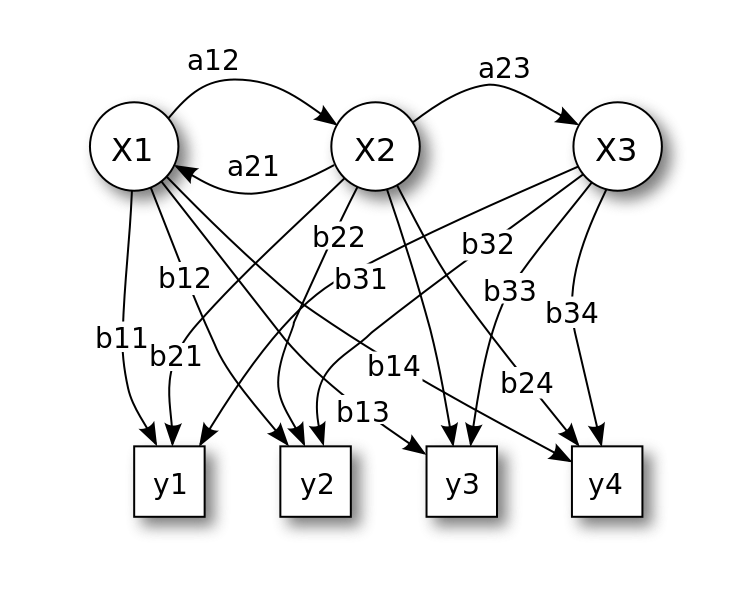
\includegraphics[width=0.5\textwidth]{hmmwiki.png}
    \caption{General Representation of a Hidden Markov Model. In this image, nodes labeled $x$ represent the states ($Q$), while those labeled $y$ represent the observations ($O$). The lines with the label $a$ represent the transition probabilities between states, and those labeled $b$ represent the probability that each of the connected observations are associated with connected states.}
    \label{fig:hmm}
\end{figure}
\RP{I HAVE TO REBUILD THIS PICTURE SO THE VARIABLE ARE THE SAME}
In our implementation, we employ two separate HMMs in order to capture the different behaviors performed by the vehicle. In the first HMM, the observations are as follows:
\begin{enumerate}
    \item Speeding Up
    \item Slowing Down
    \item Maintaining
\end{enumerate}

These observations are made using distances obtained from sensor data. In this HMM, the states are $n$ velocities $v_1,v_2,...v_{n}$ The transition matrix is a square matrix with dimension $n$ that describes how likely it is to transition from one velocity to another.

The second HMM captures the fact that vehicles can not only change their speed but also the direction in which they are travelling. In this model, the observations we make relate to the distance, $\delta$ between the vehicle and some obstacle, at which an directional change occurs:
\begin{enumerate}
    \item $\delta_1$
    \item $\delta_2$
    \item $\delta_3$... $\delta_n$
\end{enumerate}

The states in this second model, represent the directional change made: left, right, or center. We assume that this vehicle is averse to collisions, and therefore are able to limit the possible directional changes in our training and prediction.

In order to train this model, a large training period is set such that the sample is rich enough for accurate evaluation. The second HMM, in particular, can suffer from lack of enough data. The size of this period is dependent on the size of the evaluation period, which varies based on the implementation. The output of training the models are two matrices, $A$ and $B$. These matrices are built by counting the occurrences of the transition and observations associated with each state change \RP{I need an equation here - I need some help with that. I'm not sure how to show multiple iterations without algorithm}. The transition matrix for the both HMMs is a right-stochastic matrix, and satisfies the condition:

\begin{equation} \label{probsum}
    \sum_{c=1}^{n}p_{i,j} = 1
\end{equation}

where $i$ and $j$ are indices of the matrix. The observation, or emission matrices for each model are not square, but each row still meets the condition in (\ref{probsum}). Ultimately, the offline training procedure returns four matrices, $V_{tr}$, $Y_{tr}$, $V_{em}$, $Y_{em}$, representing the transition matrices for velocity and position, respectively, and the emission/observation matrices for velocity and position.



\subsubsection{Adapting Method for Online Training}
The transition and emission matrices are best returned using a large an comprehensive offline training set, but the technique can still be leveraged for online use. This is done in exactly the same manner using equation [Reference to equation I'm stuck on]. It is important, however, to note that the data set will likely return incorrect matrices at the start of runtime, as the observed vehicle will likely not have entered every state it will in the evaluation period. In order to alleviate this issue, the evaluation must begin after a certain number of states \RP{Would I call this a user parameter?} have been entered. A drawback to this method is that the prediction procedure must take place on constantly updating HMM parameters (transition and emission matrices). That being said, this capability is useful in situations where offline models do not accurately represent the observations being made, as is discussed later on in Section C. \RP{I'm not sure if this should go here or it should all move to the next section}

\subsection{Online Fitting and Prediction}
Given the two transition and two emission matrices derived from our equation, we are able to predict the future states of the observed vehicles. This is done by using the same process discussed in the previous section. The fitting process begins after one full iteration, at which point we have a state containing information about both $v$ and position, and observations from HMMs 1 and 2. We then compare these values with each of the matrices resulting from the pre-trained models as follows: Given the first observation, $o_{1}$ and first velocity $v_{1}$, we obtain the first emission probability, $b_{1}$, for each pre-trained model, $k$, we calculate

\begin{equation} \label{probdist}
   \gamma =  b_{1} - V_{em,k}(v_{1},o_{1})
\end{equation}

Where $\gamma$ represents the difference between the two probabilities. We then find the model $k$ that returns the lowest $\gamma$, denoted as $k^{*}$. Given that $k^{*}$, provides the best model for the system after the first iteration, we then apply it to the transition matrix to identify $v_{t+1}$;

\begin{equation} \label{findmaxvalue}
    v_{t+1} = \mathbf{find}\max(V_{tr,k^{*}}(v_{1},:))
\end{equation}   \RP{Not sure how to properly indicate this}

The value returned is the predicted velocity at the next iteration, and the same procedure is done for the directional HMM. However, there is significant uncertainty, as only one iteration had been used to procure this result. In order to account for this uncertainty, we perform a probabilistic assessment of each model for each HMM. For the velocity HMM, we initialize each model to have an initial probability of 
\begin{equation} \label{initprob}
    P_{k,t} = \frac{1}{K}    
\end{equation}
where $K$ is the total number of pre-trained models. With each iteration, we adjust each model in such a manner that the sum of $K$ probabilities is always equal to 1. For simplicity, we assume we know the total length of the evaluation period, $N$. We are then able to calculate the adjustment made each iteration:

\begin{equation}
    \beta = \bigg{(}\frac{1}{n}-\frac{1}{KN}\bigg{)}
\end{equation}

For the $k^{*}$, we adjust:

\begin{equation} \label{optprobadj}
    P_{k*,t+1} = P_{k*,t} + \beta
\end{equation}

For each of the remaining models $k$:

\begin{equation} \label{kprobadj}
    P_{k,t+1} = P_{k,t} - \frac{\beta}{K-1}
\end{equation}

The HMM for directional behaviors poses different challenges in probabilistic assessment. This is largely because transitions only occur when the $\delta$ approaches a certain value. As a result, the probabilities are adjusted much less frequently. The initialization is the same method as in (\ref{initprob}), adjustments, however, only occur as transitions occur in the observed vehicle. When an adjustment occurs, the comparison behaves similarly as the procedure in (\ref{probdist}) (\ref{findmaxvalue}). Until an adjustment occurs, this model is limited in its accuracy. As a result, the model that poses the most danger for the user's vehicle $i$ is assumed. This helps guarantee safe operation and will be discussed in more detail in Section D.



\subsubsection{Online HMM Fitting for Uncertain Fits}
It is possible, however, that, after performing the analyses in (\ref{optprobadj}) and (\ref{kprobadj}) there is no model whose probability exceeds a pre-set confidence level \RP{User parameter or select and justify?}. Another way this problem can arise is if the vehicle enters a state that has not been previously observed by any of the models, which would indicate library of models isn't rich enough to ensure accurate predictions.

In order to retain the fidelity of the operation, the procedure then moves to the online procedure for building a model as discussed in Section B. Because we are attempting to fit the model, rather than build a model, we have the advantage of having some baseline, the current $k^{*}$. The matrices $V_{tr,k^{*}}$, $Y_{tr,k^{*}}$, $V_{em,k^{*}}$, $Y_{em,k^{*}}$ are augmented with new states, as if they were observed in the pre-trained model. These augmented parameters are then used for real-time predictions, and are evaluated in the manner outlined earlier in this section. A drawback to this method is that the computational impact increases, as the dimensions of the parameters of the HMMs are constantly changing, requiring more intensive computation at each iteration. \RP{I think I need some more math here, I'm not sure how to show that yet}


\subsection{Risk Estimation based on Online Prediction}



\subsection{Adaptive User Assistance}


 
 
 
	



\section{Simulations}
The simulations for this work primarily occurred in Matlab. Different case-studies were performed to indicate the ability of this system to perform under varying conditions. The first case study entails a simple response to a minimally dangerous situation, the second case study involves a more complicated situation, where a safe option is clearly available. In the third case study, we examine a situation where a clearly safe option is not present, and risk is still minimized.
\subsection{Case Study 1: Simple Lane Change Behavior}
In this case, the host vehicle in the center lane responds to the actions and future position of a vehicle in the left lane, which is passing a stationary obstacle. The two snapshots of the simulation in Fig.\ref{fig:cs1} and Fig.\ref{fig:cs1b} snapshots indicate the behaviors that are occurring.

\begin{figure}[ht]
    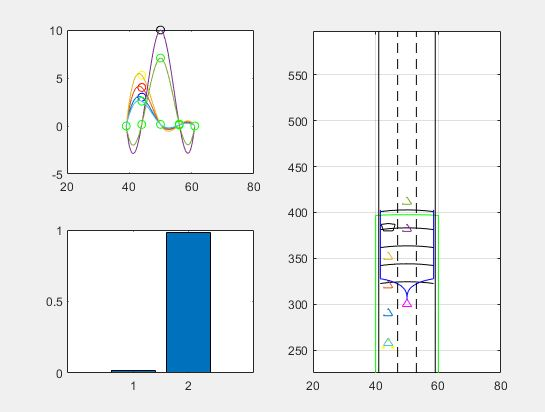
\includegraphics[width=0.5\textwidth]{cs1.JPG}
    \caption{In this snapshot, $u_{\alpha} = 0$ and $u_{h} = 1$. This is because the risk in the vehicle's current lane at $t = t+3$ is well below the $\lambda_{r}$.}
    \label{fig:cs1}
\end{figure}

\begin{figure}[ht]
    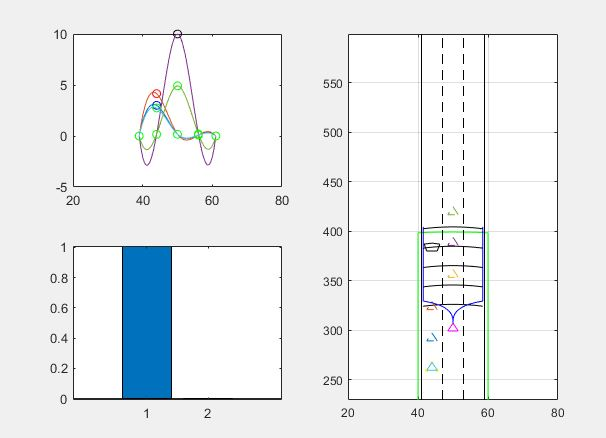
\includegraphics[width=0.5\textwidth]{cs1b.JPG}
    \caption{In this snapshot, the risk in the host vehicle's lane at $t+3$ has increased above $\lambda_{r}$, and autonomy has increased rapidly. The reason $u_{alpha}$ has increased to 1, is because this is the instant at which the change begins. The location of minimum risk is determined to be the right lane, and the vehicle will then move to the right lane.}
    \label{fig:cs1b}
\end{figure}

This simulation results in a safe operation, as the minimum risk is easily identified and the solution is offered. In this simulation, the human takes no action, which is another reason fully autonomous intervention occurs, and the risk is still minimized and avoided.

\subsection{Case Study 2: Dynamic Environment with Lane Change Behavior}
In the second simulation, the human does take some action and it is evident that autonomy and human-control are fluid and change based on changing surroundings. In addition, there is once again a clear location at which the risk is at a minimum. The snapshot in Fig.\ref{fig:cs2} shows a situation where the user is travelling at a velocity slightly too rapid for the obstacle ahead, and slowing down will not put it at a risky position in relation to the next vehicle that is behind the user. As a result, $u_{\alpha}$ is increased as the level of risk increases.
\begin{figure}[ht]
    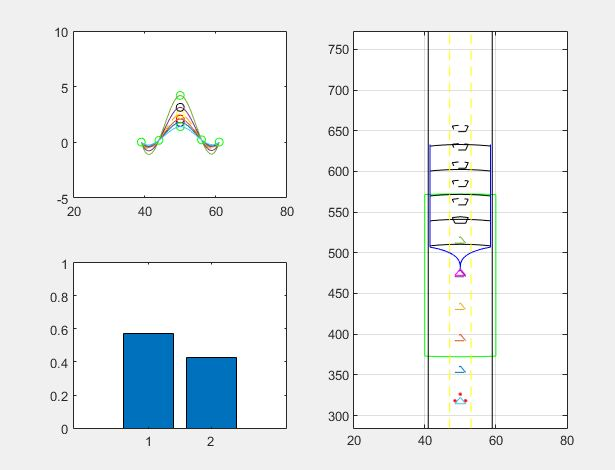
\includegraphics[width=0.5\textwidth]{cs2.JPG}
    \caption{In this snapshot, $u_{\alpha} > u_{h}$. This is because the risk in the vehicle's current lane at $t = t+3$ is slightly above the $\lambda_{r}.$}
    \label{fig:cs2}
\end{figure}
This result also indicates a case of the user's desires being met as closely as possible. The user, by not only adjusting velocity and not adjusting their lane change behavior, indicates that the velocity is the first parameter to adjust. As shown in Fig.\ref{fig:cs2c}, the velocity is only adjusted so that the driver is in a safe position for the selected $t+3$ time and, consequently for times $t+1$ and $t+2$. This is indicated by a velocity that slowly decreases to a safe value. This, however, would only suffice to maximize the time before a collision occurs. Because that is a limitation of only adjusting the velocity, when a collision becomes imminent, $u_\alpha$ increase to 1, and the lane is changed to that of minimum risk.
\begin{figure}[ht]
    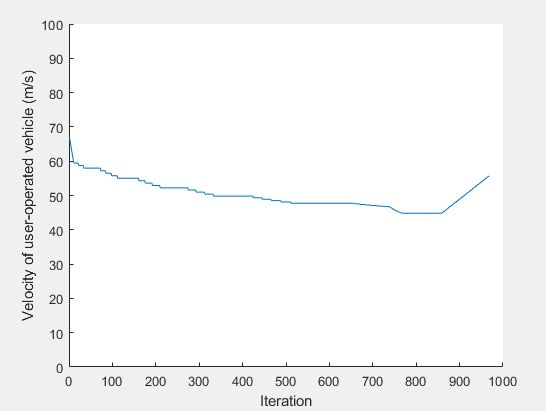
\includegraphics[width=0.5\textwidth]{cs2c.JPG}
    \caption{This figure depicts the velocity of the user's vehicle}
    \label{fig:cs2c}
\end{figure}

\subsection{Case Study 3: Highly dangerous situation with limited options.}
The third case is built much like the second case. In this implementation, however, neither of the two surrounding lanes are available. In this case, the system begins to react much like that of the second case, however, there is a error in the prediction of what the following vehicle will do. This is because the model was trained for a lane change, but it is evident that a lane change will not occur when the actual vehicle (not the estimates) approaches our user's vehicle. An adjustment of the velocities in this case are shown in \ref{fig:vehiclepos}. In a situation like this, the algorithm does delay the imminent collision, but there is a specific preference to retain a certain following distance, $\Delta d$ behind the obstacle in front. We assume that the user's vehicle has a responsibility to not directly cause a collision on its own. This does, however, leave the possibility of a rear collision.




\section{Experiment}
\section{Conclusions}

\newpage
% references section

% can use a bibliography generated by BibTeX as a .bbl file
% BibTeX documentation can be easily obtained at:
% http://mirror.ctan.org/biblio/bibtex/contrib/doc/
% The IEEEtran BibTeX style support page is at:
% http://www.michaelshell.org/tex/ieeetran/bibtex/
%\bibliographystyle{IEEEtran}
% argument is your BibTeX string definitions and bibliography database(s)
%\bibliography{IEEEabrv,../bib/paper}
%
% <OR> manually copy in the resultant .bbl file
% set second argument of \begin to the number of references
% (used to reserve space for the reference number labels box)

%\begin{thebibliography}{1}

%\bibitem{IEEEhowto:kopka}
%H.~Kopka and P.~W. Daly, \emph{A Guide to \LaTeX}, 3rd~ed.\hskip 1em %plus
%  0.5em minus 0.4em\relax Harlow, England: Addison-Wesley, 1999.
  
  
%\end{thebibliography}

%\printbibliography
\bibliographystyle{abbrv}
\bibliography{mybibliography}


% that's all folks
\end{document}


